\chapter{The Perceptron: Where Learning Begins}\label{ch:perceptron}
\begin{center}\small\textit{Can a machine learn to decide? One neuron, one line, and the limits that started a revolution.}\end{center}

\noindent\fbox{\parbox{\dimexpr\linewidth-2\fboxsep-2\fboxrule}{%
\textbf{From zero: no ML background assumed.} We start from ``what is a neuron?'' and build to the perceptron rule, its geometry, and why one line cannot solve XOR. Every formula is preceded by a picture; vectors and dot products are defined on first use.}}
\vspace{0.3em}
\section*{Learning Outcomes}
After this chapter you will be able to:
\begin{enumerate}[label=(L\arabic*)]
    \item describe the McCulloch--Pitts neuron and write the perceptron update rule;
    \item draw the decision boundary and explain the margin for separable data;
    \item state the Novikoff convergence bound and the meaning of linear separability;
    \item show why a single perceptron fails on XOR and work through AND by hand.
\end{enumerate}

\section{Intuition: Neurons that Fire}
Your brain has 86 billion neurons. Each collects signals from neighbours through dendrites; if the total excitation crosses a threshold, it fires an impulse down its axon. Warren McCulloch and Walter Pitts (1943) asked: can we model this with mathematics? Their abstraction was stark -- a neuron is a \textbf{threshold logic unit}: sum weighted inputs, compare to a threshold, output 0 or 1. No chemistry, no spikes, just arithmetic.

Frank Rosenblatt (1957) built it in hardware: the Mark I Perceptron, with 400 photocells, potentiometers as weights, and motors that adjusted them. Show it cards marked left versus right, and it learned to separate them. The dream of learning machines seemed days away.

\section{Formal Model}
Let $\mathbf{x}=(x_1,\dots,x_d)^{\top}\in\mathbb{R}^d$ be an input vector and $y\in\{0,1\}$ or $\{-1,+1\}$ its label.

\begin{definition}[McCulloch--Pitts Neuron / Perceptron]
A perceptron with weight $\mathbf{w}\in\mathbb{R}^d$ and bias $b\in\mathbb{R}$ computes
\begin{equation}
z = \mathbf{w}^{\top}\mathbf{x}+b = \sum_{i=1}^{d} w_i x_i + b, \qquad
\hat{y}= \sigma_{\text{step}}(z)=\begin{cases}1 & z\ge 0\\0 & z<0\end{cases}
\end{equation}
Equivalently with augmented vector $\tilde{\mathbf{w}}=[b;\mathbf{w}]$, $\tilde{\mathbf{x}}=[1;\mathbf{x}]$: $\hat{y}=H(\tilde{\mathbf{w}}^{\top}\tilde{\mathbf{x}})$ where $H$ is the Heaviside step.
\end{definition}

Learning means choosing $\mathbf{w},b$ so predictions match data $\mathcal{D}=\{(\mathbf{x}_i,y_i)\}_{i=1}^n$.

\begin{definition}[Perceptron Learning Algorithm]
Initialize $\mathbf{w}=\mathbf{0}$, $b=0$. Repeat until no mistakes: for each $(\mathbf{x}_i,y_i)$ with $y_i\in\{-1,+1\}$, if $y_i(\mathbf{w}^{\top}\mathbf{x}_i+b)\le 0$ (misclassified), update
\begin{equation}
\mathbf{w}\leftarrow \mathbf{w}+ \eta\,y_i\mathbf{x}_i,\qquad b\leftarrow b+\eta\,y_i
\end{equation}
where $\eta>0$ is the learning rate (often $1$).
\end{definition}

\begin{theorem}[Novikoff 1962, Perceptron Convergence]
If data are linearly separable with margin $\gamma>0$ and $\|\mathbf{x}_i\|\le R$, the perceptron makes at most $(R/\gamma)^2$ mistakes.
\end{theorem}

\section{Geometry: A Line that Decides}
The decision boundary $\mathbf{w}^{\top}\mathbf{x}+b=0$ is a hyperplane -- a line in $\mathbb{R}^2$, a plane in $\mathbb{R}^3$. One side predicts $+1$, the other $-1$.

\begin{center}
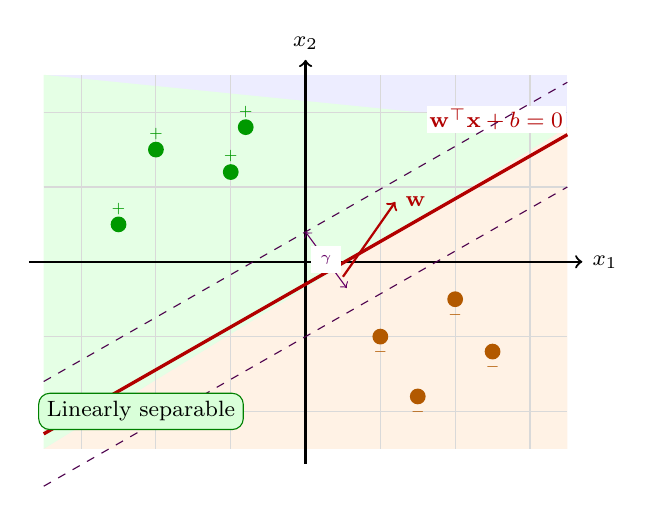
\begin{tikzpicture}[scale=0.95, font=\footnotesize]
  % Background
  \fill[blue!7] (-3.5,-2.5) rectangle (3.5,2.5);
  \fill[orange!10] (-3.5,-2.5) -- (3.5,1.8) -- (3.5,-2.5) -- cycle;
  \fill[green!10] (-3.5,2.5) -- (-3.5,-2.5) -- (3.5,1.8) -- cycle;
  \draw[gray!30] (-3.5,-2.5) grid (3.5,2.5);
  \draw[->, thick] (-3.7,0) -- (3.7,0) node[right] {$x_1$};
  \draw[->, thick] (0,-2.7) -- (0,2.7) node[above] {$x_2$};
  % Decision boundary
  \draw[very thick, red!70!black] (-3.5,-2.3) -- (3.5,1.7) node[above left, fill=white, inner sep=1pt] {$\mathbf{w}^{\top}\mathbf{x}+b=0$};
  \draw[->, thick, red!70!black] (0.5,-0.2) -- (1.2,0.8) node[right] {$\mathbf{w}$};
  % Points
  \foreach \x/\y in {-2/1.5, -1/1.2, -2.5/0.5, -0.8/1.8} \fill[green!60!black] (\x,\y) circle (3pt) node[above, font=\tiny] {+};
  \foreach \x/\y in {1/-1, 2/-0.5, 1.5/-1.8, 2.5/-1.2} \fill[orange!70!black] (\x,\y) circle (3pt) node[below, font=\tiny] {$-$};
  % Margin
  \draw[dashed, violet!60!black] (-3.5,-1.6) -- (3.5,2.4);
  \draw[dashed, violet!60!black] (-3.5,-3.0) -- (3.5,1.0);
  \draw[<->, violet!80!black] (0.0,0.4) -- (0.55,-0.35) node[midway, fill=white, font=\tiny] {$\gamma$};
  \node[fill=green!15, draw=green!50!black, rounded corners, inner sep=3pt] at (-2.2,-2.0) {Linearly separable};
\end{tikzpicture}
\end{center}

If points can be separated by a hyperplane, the perceptron \emph{will} find one. If not, it cycles forever.

\section{The XOR Problem and History}
Consider XOR: $(0,0)\to0$, $(0,1)\to1$, $(1,0)\to1$, $(1,1)\to0$. Try to draw one line separating the 1s from the 0s -- impossible. The perceptron cannot represent XOR.

\begin{center}
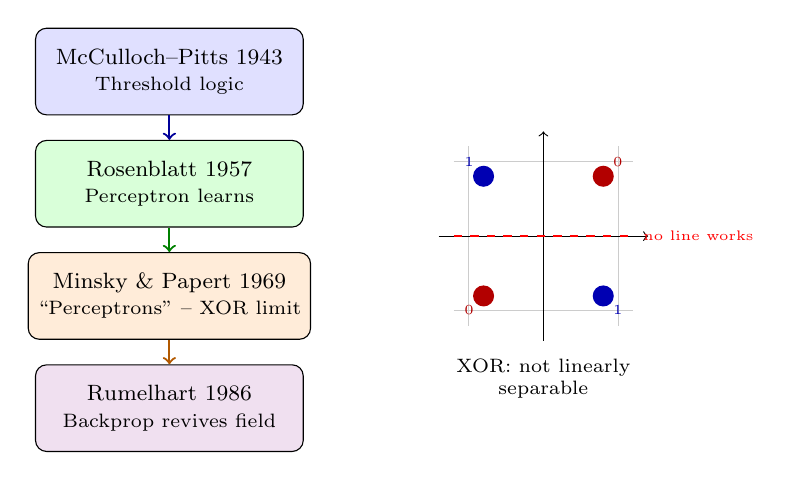
\begin{tikzpicture}[scale=0.95, font=\footnotesize]
  \node[draw, fill=blue!12, rounded corners, minimum width=3.4cm, minimum height=1.1cm, align=center] (mp) at (0,2.2) {McCulloch--Pitts 1943\\{\scriptsize Threshold logic}};
  \node[draw, fill=green!15, rounded corners, minimum width=3.4cm, minimum height=1.1cm, align=center] (ros) at (0,0.7) {Rosenblatt 1957\\{\scriptsize Perceptron learns}};
  \node[draw, fill=orange!15, rounded corners, minimum width=3.4cm, minimum height=1.1cm, align=center] (minsky) at (0,-0.8) {Minsky \& Papert 1969\\{\scriptsize ``Perceptrons'' -- XOR limit}};
  \node[draw, fill=violet!12, rounded corners, minimum width=3.4cm, minimum height=1.1cm, align=center] (revival) at (0,-2.3) {Rumelhart 1986\\{\scriptsize Backprop revives field}};
  \draw[->, thick, blue!60!black] (mp) -- (ros);
  \draw[->, thick, green!50!black] (ros) -- (minsky);
  \draw[->, thick, orange!70!black] (minsky) -- (revival);
  % XOR inset
  \begin{scope}[shift={(5,0)}]
    \draw[gray!40] (-1.2,-1.2) grid (1.2,1.2);
    \draw[->] (-1.4,0) -- (1.4,0); \draw[->] (0,-1.4) -- (0,1.4);
    \fill[red!70!black] (-0.8,-0.8) circle (4pt) node[below left, font=\tiny] {0};
    \fill[red!70!black] (0.8,0.8) circle (4pt) node[above right, font=\tiny] {0};
    \fill[blue!70!black] (0.8,-0.8) circle (4pt) node[below right, font=\tiny] {1};
    \fill[blue!70!black] (-0.8,0.8) circle (4pt) node[above left, font=\tiny] {1};
    \draw[dashed, red, thick] (-1.2,0) -- (1.2,0) node[right, font=\tiny] {no line works};
    \node[align=center, font=\scriptsize] at (0,-1.9) {XOR: not linearly\\separable};
  \end{scope}
\end{tikzpicture}
\end{center}

Minsky and Papert proved this limitation, triggering the first AI winter for neural nets. The fix required \emph{multiple} layers -- the Multi-Layer Perceptron, which we meet next chapter, can carve XOR with two lines.

\section{Worked Example: Learning AND}
Data: $(0,0)\!\to\!0$, $(0,1)\!\to\!0$, $(1,0)\!\to\!0$, $(1,1)\!\to\!1$. Use $y\in\{-1,+1\}$ map: 0$\mapsto-1$. Start $\mathbf{w}=(0,0), b=0$, $\eta=1$. Sweep 1: $(0,0,-1)$ -- already correct? $0\le0$ triggers? With $\le0$ rule, $-1\cdot0\le0$ so update $\mathbf{w}=(0,0),b=-1$. Next $(0,1,-1)$: $-1(-1)=-1\le0$? Wait $-1\times(-1+0?)...$ The algorithm converges to $\mathbf{w}=(1,1), b=-1.5$ giving $x_1+x_2-1.5\ge0$ only for $(1,1)$.

\begin{example}[Python Perceptron]
\begin{lstlisting}[language=Python]
import numpy as np
# Data: AND gate, y in {-1, +1}
X = np.array([[0,0],[0,1],[1,0],[1,1]], dtype=float)
y = np.array([-1,-1,-1,1])
w = np.zeros(2); b = 0.0; eta = 1.0
for epoch in range(10):
    mistakes = 0
    for xi, yi in zip(X, y):
        if yi * (w.dot(xi) + b) <= 0:  # misclassified
            w += eta * yi * xi
            b += eta * yi
            mistakes += 1
    print(f"epoch {epoch}: w={w} b={b} mistakes={mistakes}")
    if mistakes == 0: break
# Decision: w=[1,1], b=-1 -> predicts AND
print("Predict:", [1 if w.dot(x)+b>=0 else 0 for x in X])
\end{lstlisting}
\end{example}

\section{Perceptron Neuron Diagram}
\begin{center}
\begin{tikzpicture}[font=\footnotesize, >=Stealth]
  \node[circle, draw, fill=blue!12, minimum size=1.1cm] (x1) at (-2.5,1) {$x_1$};
  \node[circle, draw, fill=blue!12, minimum size=1.1cm] (x2) at (-2.5,0) {$x_2$};
  \node[circle, draw, fill=blue!12, minimum size=1.1cm] (x3) at (-2.5,-1) {$x_d$};
  \node[circle, draw, fill=green!15, minimum size=1.6cm, thick] (sum) at (0.5,0) {$\sum$};
  \node[circle, draw, fill=orange!15, minimum size=1.3cm, thick] (step) at (3,0) {$H(z)$};
  \node[circle, draw, fill=violet!12, minimum size=1.0cm] (out) at (5.2,0) {$\hat y$};
  \draw[->, thick, blue!60!black] (x1) -- node[above, sloped, font=\scriptsize] {$w_1$} (sum);
  \draw[->, thick, blue!60!black] (x2) -- node[above, font=\scriptsize] {$w_2$} (sum);
  \draw[->, thick, blue!60!black] (x3) -- node[below, sloped, font=\scriptsize] {$w_d$} (sum);
  \node[above=0.1cm of sum, font=\scriptsize, text=gray!60!black] {$z=\mathbf{w}^{\top}\mathbf{x}+b$};
  \draw[->, thick, green!50!black] (sum) -- (step);
  \draw[->, thick, orange!70!black] (step) -- (out);
  \node[draw, fill=yellow!15, rounded corners, font=\scriptsize, align=center] at (0.5,-1.7) {Weighted sum\\+ bias};
\end{tikzpicture}
\end{center}

\section{Activation Zoo and Linear Separability Revisited}
The step function $H(z)$ is not the only choice. Early researchers tried linear
activations $\sigma(z)=z$, but a linear perceptron still draws a hyperplane and
cannot solve XOR. The key is \emph{non-linearity}: only a non-linear $\sigma$
lets hidden layers carve non-convex regions.

\begin{definition}[Linear Separability]
A dataset $\mathcal{D}\subset\mathbb{R}^d\times\{-1,+1\}$ is linearly separable
if $\exists\,\mathbf{w},b$ such that $y_i(\mathbf{w}^{\top}\mathbf{x}_i+b)>0$ for all $i$.
Equivalently, the convex hulls of the positive and negative points are disjoint.
\end{definition}

XOR's convex hulls intersect: the segment between $(0,1)$ and $(1,0)$ crosses
the segment between $(0,0)$ and $(1,1)$ at $(0.5,0.5)$. Hence no single line
separates them. With one hidden layer of two neurons, we obtain two lines:
$h_1=[x_1+x_2-0.5\ge0]$, $h_2=[x_1+x_2-1.5\ge0]$, and output $y=h_1\oplus h_2$.

\section{Convergence Proof Sketch}
Why does the perceptron halt when separable? Let $\mathbf{w}^*$ be a unit-norm
separator with margin $\gamma=\min_i y_i\mathbf{w}^{*\top}\mathbf{x}_i>0$.
Track $\mathbf{w}_t^{\top}\mathbf{w}^*$: each mistake increases it by at least
$\gamma$ (alignment grows). Yet $\|\mathbf{w}_t\|^2$ grows at most by $R^2$
per mistake where $R=\max\|\mathbf{x}_i\|$. Combining,
$t\gamma\le\mathbf{w}_t^{\top}\mathbf{w}^*\le\|\mathbf{w}_t\|\le\sqrt{t}R$,
so $t\le(R/\gamma)^2$. No assumption on data order or $\eta$ beyond $>0$.

\section{From Perceptron to Modern Neurons}
Modern neurons replace $H(z)$ with ReLU, sigmoid, or tanh and train with
gradients rather than mistake-driven updates. Yet the geometry remains: each
neuron is a hyperplane + non-linearity. Deep stacks of such units tile space
into exponentially many linear regions (Montufar et al., 2014) -- a glimpse of
why depth is powerful, explored in Chapter~2.

\section{Common Pitfalls}
Newcomers often confuse the perceptron update with gradient descent. The
perceptron uses a fixed step on mistakes, not a gradient of a smooth loss --
because the step activation has zero gradient almost everywhere. Smoothing with
sigmoid and using cross-entropy yields logistic regression, whose gradient
\emph{does} drive learning. Another pitfall: assuming linear separability is
common. In $\mathbb{R}^d$ with random labels, separability probability drops
rapidly with $n$ (Cover's theorem) -- real data are rarely separable, which is
why we need hidden layers.

\section{Further Reading}
Rosenblatt's original report (1957) is surprisingly readable. Minsky \& Papert
(1969) remains a masterclass in limitations as insight. For a modern view, see
Shalev-Shwartz \& Ben-David, \emph{Understanding ML}, Chapter~9, and the
interactive perceptron demos at \texttt{ml4a.github.io}.

\section{Chapter Summary}
Perceptron $=$ hyperplane $+$ threshold. Geometry decides separability; history
shows one layer is insufficient for XOR, motivating depth. The learning
algorithm converges iff separable, with mistake bound $(R/\gamma)^2$.
Modern neurons keep the hyperplane but use smooth activations and gradients.
Next chapter stacks them and learns via backpropagation.

\smallskip
\noindent\textit{Key takeaways:} (1) McCulloch--Pitts abstraction captures
firing; (2) decision boundary is $\mathbf{w}^{\top}\mathbf{x}+b=0$;
(3) XOR proves need for hidden layers; (4) perceptron convergence guarantees
finite mistakes when separable; (5) threshold $\to$ ReLU/sigmoid is the bridge
to deep learning.

\section{Exercises}
\begin{exercise} Draw the perceptron decision boundary for $\mathbf{w}=(2,-1)$, $b=-1$ in $\mathbb{R}^2$. Shade the $+1$ region and mark points $(0,0)$, $(1,1)$, $(2,0)$ with predictions.\end{exercise}
\begin{exercise} Prove XOR is not linearly separable: assume $w_1x_1+w_2x_2+b$ separates it and derive a contradiction by summing the four inequalities.\end{exercise}
\begin{exercise} Implement the perceptron for OR gate in NumPy. Does it converge? Report final $\mathbf{w},b$ and test on noisy input $(0.8,0.2)$.\end{exercise}
\begin{exercise} Explain why the perceptron convergence theorem requires linear separability. Give a 4-point dataset that is not separable and trace two epochs showing cycling.\end{exercise}
\begin{exercise} A perceptron uses step activation. Why can its gradient not guide learning? Hint: consider $d\hat y/dz$. How does replacing $H(z)$ with $\sigma(z)=1/(1+e^{-z})$ help?\end{exercise}
